%%%%%%%%%%%%%%%%%%%%%%%%%%%%%%%%%%%%%%%%%%

\section{Results of the cut-based analysis}

\label{sec:results}

In this section we present the results of the 
cut-based analysis and
compare our results with other recent related studies.
%
We study how the signal significance
is modified if only the $4b$ component of the
QCD multi-jet background is taken into account,
but the $2b2j$ and $4j$ components are neglected.
%


\subsection{Cut flow and signal significance}

First of all we compare the cross-sections at various
analysis levels for the three categories, for signal and background events,
by providing a detailed cut-flow.
%
We consider all backgrounds enumerated in Sect.~\ref{mcgeneration},
then we discuss how results are modified if only the $4b$
component is kept.
%
we consider the following levels of the cut-flow
\begin{itemize}
\item {\bf C0}: cross-sections at the generator
  level, before any analysis cuts.
\item {\bf C1}:  cross-sections after the basic jet acceptance selection
  cuts, but before $b$-tagging.
\item {\bf C2}: cross-sections after after the $b$-tagging.
\end{itemize}
Note that {\bf C1} already includes the effect of the Higgs mass
window cut, Eq.~(\ref{higgsmasswindow}).
%
At the {\bf C0} level the numbers will be the same
for the three individual categories.

In the following, results are presented for the exclusive
categorisation defined in Sect.~\ref{sec:categorisation}.
%
%
At each stage of the cut flow, we also provide the number
of events that would be expected at the HL-LHC with
an integrated luminosity of $\mathcal{L}_{\rm int}
=3000$ fb$^{-1}$,
as well as 
the signal significance $S/\sqrt{B}$ and the signal
over background ratio $S/B$.
%
We emphasize that it is important not only to achieve a good signal
significance, $S/\sqrt{B}$, but also a good signal over background ratio $S/B$:
if the latter is too small, a very accurate
measurement of the background with an infeasible small
systematic uncertainty would be required.


%%%%%%%%%%%%%%%%%%%%%%%%%%%%%%%%%%%%%%%%%%%%%%%%%%%%%
\begin{table}[t]
  \centering
  \begin{tabular}{c|c|c||c|c||c|c}
    \hline
    \multicolumn{7}{c}{Boosted category}\\
    \hline
    \hline
    &    \multicolumn{2}{c||}{$\sigma$ (fb)}   &  \multicolumn{2}{c||}{$N_{\rm ev}$}
    &   $S/\sqrt{B}$  & $S/B$\\
      &    Signal & Back   &  Signal  & Back
    &   & \\
    \hline
        {\bf C0}  &  36.9  & $9.9\,10^{9}$ & $1.1\,10^5$ & $3.0\,10^{13}$  &  0.020 & $3.7\,10^{-9}$\\
        {\bf C1}  &  0.46    & $1.3\,10^6$    &  $1.4\,10^3$   & $3.9\,10^9$     & 0.022     &  $3.5\,10^{-7}$ \\
        {\bf C2}  &  0.064     &  12.6     &  193   &  $3.8\,10^4$    &  0.99    &  $5.1\,10^{-3}$ \\
        \hline
  \end{tabular}
  $\,$\\
  \vspace{0.4cm}
  \begin{tabular}{c|c|c|c|c|c|c}
    \hline
    \multicolumn{7}{c}{Intermediate category}\\
    \hline
    \hline
    &    \multicolumn{2}{c|}{$\sigma$ (fb)}   &  \multicolumn{2}{c|}{$N_{\rm ev}$}
    &   $S/\sqrt{B}$  & $S/B$\\
      &    Signal & Back   &  Signal  & Back
    &   & \\
    \hline
         {\bf C0}  &  36.9  & $9.9\,10^{9}$ & $1.1\,10^5$ & $3.0\,10^{13}$  &  0.020 & $3.7\,10^{-9}$\\
        {\bf C1}  &   1.44    &   $1.1\,10^{7}$  &  $4.3\,10^3$   &  $3.3\,10^{10}$    &  0.024    &  $1.3\,10^{-7}$ \\
        {\bf C2}  &   0.22    &  722   &  660   &   $2.2\,10^6$   &   0.45   &  $3.1\,10^{-4}$ \\
        \hline
  \end{tabular}
  $\,$\\
  \vspace{0.4cm}
  \noindent
  \begin{tabular}{c|c|c|c|c|c|c}
    \hline
    \multicolumn{7}{c}{Resolved category}\\
    \hline
    \hline
    &    \multicolumn{2}{c|}{$\sigma$ (fb)}   &  \multicolumn{2}{c|}{$N_{\rm ev}$}
    &   $S/\sqrt{B}$  & $S/B$\\
      &    Signal & Back   &  Signal  & Back
    &   & \\
    \hline
       {\bf C0}  &  36.9  & $9.9\,10^{9}$ & $1.1\,10^5$ & $3.0\,10^{13}$  &  0.020 & $3.7\,10^{-9}$\\
        {\bf C1}  &   3.34    & $7.5\,10^{7}$    & $1.1\,10^4$    & $3.3\,10^{10}$     & 0.021     & $4.5\,10^{-8}$  \\
        {\bf C2}  &   0.54    &  $3.5\,10^{3}$   &  $1.6\,10^{3}$   &   $1.1\,10^{7}$   & 0.50     &  $1.5\,10^{-4}$ \\
        \hline
  \end{tabular}
  \caption{\small Cut-flow for the analysis of the boosted (top),
    intermediate (middle) and resolved (bottom)
    categories.
    %
    At each level of the cut-flow, we indicate the cross-sections and the number of
    expected events at the HL-LHC for $\mathcal{L}_{\rm int}=3$ ab$^{-1}$, both for
    signal events and for all the backgrounds combined.
    %
    We also provide in each case the
    signal significance $S/\sqrt{B}$ and the signal
    over background ratio $S/B$.
    %
    The first row {\bf C0} is the generator-level result and thus is common
    to all three categories.
    %
    \label{table:cutflow}
  }
\end{table}
%%%%%%%%%%%%%%%%%%%%%%%%%%%%%%%%%%%%%%%%%%%%%%%%%%%%%


The results for the three categories have been collected in
Table~\ref{table:cutflow}.
%
Let us begin with the discussion of the boosted category, the one that
leads to a higher signal significance.
%
We see that after all the cuts, including $b$-tagging,
we end up with almost 200 signal events at the HL-LHC, with
still a substantial background of around $40k$ events.
%
The signal significance is around 1.0 at the end of the
cut-based analysis.
%
While it should have been possible to increase this significance
but using more aggressive cuts, we have refrained doing so
since we prefer this optimisation to be performed at the level of
the MVA.


From the results of Table~\ref{table:cutflow}
it is possible to compute the corresponding numbers
for the end of Run II at the LHC with
$\mathcal{L}_{\rm int}=300$ fb$^{-1}$: in the boosted category,
we have only
19 signal events, and the signal significance drops down to
$S/\sqrt{B}\sim 0.3$.
%
We will discuss in the next section what are the Run II prospects
once we include the effects of the MVA in the analysis, but
it is clear already at this level that one really needs the full
integrated luminosity of the HL-LHC to be able to observe
the Higgs pair production process, unless  of course production rates are
increased by new BSM dynamics

Both the intermediate and resolved categories benefit from higher signal yields,
specially in the resolved category, but this enhancement is washed out by the stronger
increase in the QCD multi-jet background.
%
In both cases the signal significance is around half of that in the boosted category,
with in addition $S/B$ being an order of magnitude smaller.
%
Therefore, the boosted category is clearly determined to be the most useful category,
specially due to the significant suppression of the QCD multi-jet background.
%
And we still have not exploited all the rich information contained on the jet
substructure, as we will do in the next section.

From the results of Table~\ref{table:cutflow}
we see that after the cut-based analysis, the significance of the Higgs pair production
observation in the $4b$ channel using the boosted topology
is $S/\sqrt{B}=0.99$,
and that the combination
of the boosted, intermediate and resolved categories gives a slightly higher
value, around 1.20.
%

\subsection{Comparison with previous work}

The feasibility of Higgs pair production at the HL-LHC in different
final-state channels
has been explored various groups~\cite{Baur:2003gp,Barger:2013jfa,
  Baur:2003gpa,Barr:2013tda,Dolan:2013rja,
  Dolan:2012rv,Papaefstathiou:2012qe,Gouzevitch:2013qca,Cooper:2013kia,Wardrope:2014kya,deLima:2014dta}, though
the $4b$ final state has received less attention than other final states,
due to the complexity of disentangling the signal over the large
QCD multijet background.
%
Now we compare with two recent studies that have also studied the
feasibility of SM Higgs pair production in the $4b$ final state,
those of the UCL group~\cite{Wardrope:2014kya} and of the
Durham group~\cite{deLima:2014dta}.
%
In order to perform a meaningful comparison, we will only consider
here the $4b$ QCD and $t\bar{t}$ backgrounds, as was done
in these two studies.

First of all let us briefly summarize these two studies.
%
In the UCL group study~\cite{Wardrope:2014kya} is based
on requiring at least four $b$-tagged $R=0.4$ anti-$k_T$ jets
in the central acceptance with $p_T \ge 40$ GeV, which are
then used to form dijets (Higgs candidates) with
$p_T \ge 150$ GeV, $85 \le m_{\rm dijet} \le 140$ GeV
and $\Delta R \le 1.5$ between the two jets that form
each dijet system.
%
In addition to the basic selection cuts, a large number
of additional variables are combined using a
Boosted Decision Tree (BDT) discriminant.
%
This study considers the $b\bar{b}b\bar{b}$ and
$b\bar{b}c\bar{c}$ QCD multijets as well as
$t\bar{t}$, $Zh$, $t\bar{t}h$ and $hb\bar{b}$.
%
Their final significance is found to the $S/\sqrt{B}=2.1$ at the HL-LHC.

The Durham group study~\cite{deLima:2014dta} requires events
to have two $R=1.2$ C/A jets with $p_T\ge 200$ GeV, with
two $b$-tagged subjets inside each large-$R$ jet with
$p_T \ge$ 40 GeV.
%
To improve the signal over background separation, both the BDRS
method and the Shower Deconstruction (SD)~\cite{Soper:2011cr,Soper:2012pb}
technique are applied.
%
The background considered are QCD $4b$ as well as $Zb\bar{b}$, $hZ$ and
$hW$, but no $t\bar{t}$, $2b2j$ or $4j$.
%
At the HL-LHC, the best performance is obtained by requiring two
SD-tagged large-$R$ jets, which leads to $S/\sqrt{B}\sim 2.1$,
with BDRS similar but slightly inferior performance.
%
Therefore, both the Durham and the UCL groups conclude that a signal
significance $S/\sqrt{B}$ slightly above two can  be obtained
in this channel at the HL-LHC.

Since we find that the $2b2j$ and $4j$ backgrounds cannot
be neglected, and previous works did not considered them,
it is interesting to
study how our results are modified if we consider only the QCD $4b$
multi-jet background, but ignore the $2b2j$ and $4j$ backgrounds,
that is, we ignore the contribution from the fakes.
%
These results are shown in
Table~\ref{table:cutflow4B}, which is the analog of
Table~\ref{table:cutflow} but with only the QCD
$4b$ background taken into account.
%
As we can see, these results indicate that given the similarity of the final states
in signal and background events in these cases, the signal significance is
relatively stable at various stages of the cut-flow.
%
As compared to the case in which all backgrounds are taken into account, we
now get a factor two smaller backgrounds: we conclude that in the boosted category
the effect of the fakes is non-negligible, with their contribution being
comparable to that of the irreducible $4b$ QCD multi-jet background.

Concerning the other categories, we see that that ignoring the fakes can lead to a substantial
distortion of the results.
%
In the intermediate category, the signal significance is now much better, with $S/\sqrt{B}$ increasing from
0.5 with all the backgrounds to $1.57$ if only $4b$ are accounted for, a factor 3 improvement.
%
Also the resolved category improves substantially, with signal significance increasing by a factor 2.
%
Therefore, we conclude that a careful modeling of the fakes is very important to truly quantify
the feasibility of Higgs pair production in the $4b$ channel, though for the most
important category, the boosted category, the results are relatively stable.
%
Moreover, we find that the effect of the multijet fake background is of
the same size of the higher-order QCD corrections to $4b$ production~\cite{Binoth:2009rv}.


%%%%%%%%%%%%%%%%%%%%%%%%%%%%%%%%%%%%%%%%%%%%%%%%%%%%%
\begin{table}[t]
  \centering
  \begin{tabular}{c|c|c||c|c||c|c}
    \hline
    \multicolumn{7}{c}{Boosted category}\\
    \hline
    \hline
    &    \multicolumn{2}{c||}{$\sigma$ (fb)}   &  \multicolumn{2}{c||}{$N_{\rm ev}$}
    &   $S/\sqrt{B}$  & $S/B$\\
      &    Signal & Back   &  Signal  & Back
    &   & \\
    \hline
        {\bf C0}  &  36.9  & $1.1\,10^{6}$ & $1.1\,10^5$ & $3.3\,10^{9}$  &  1.90 & $3.3\,10^{-5}$\\
        {\bf C1}  &  0.46    & $1.0\,10^2$    &  $1.4\,10^3$   & $3.1\,10^5$     & 2.48     &  $4.4\,10^{-3}$ \\
        {\bf C2}  &  0.064     &  7.1     &  193   &  $2.1\,10^4$    &  1.30    &  $9.1\,10^{-3}$ \\
        \hline
  \end{tabular}
   $\,$\\
  \vspace{0.4cm}
  \begin{tabular}{c|c|c|c|c|c|c}
    \hline
    \multicolumn{7}{c}{Intermediate category}\\
    \hline
    \hline
    &    \multicolumn{2}{c|}{$\sigma$ (fb)}   &  \multicolumn{2}{c|}{$N_{\rm ev}$}
    &   $S/\sqrt{B}$  & $S/B$\\
      &    Signal & Back   &  Signal  & Back
    &   & \\
    \hline
 {\bf C0}  &  36.9  & $1.1\,10^{6}$ & $1.1\,10^5$ & $3.3\,10^{9}$  &  1.90 & $3.3\,10^{-5}$\\
        {\bf C1}  &  0.46    & $7.2\,10^2$    &  $1.4\,10^3$   & $2.2\,10^6$     & 2.91     &  $1.9\,10^{-3}$ \\
        {\bf C2}  &  0.064     &  58.8     &  193   &  $1.8\,10^5$    &  1.57    &  $3.7\,10^{-3}$ \\
        \hline
  \end{tabular}
  $\,$\\
  \vspace{0.4cm}
  \noindent
  \begin{tabular}{c|c|c|c|c|c|c}
    \hline
    \multicolumn{7}{c}{Resolved category}\\
    \hline
    \hline
    &    \multicolumn{2}{c|}{$\sigma$ (fb)}   &  \multicolumn{2}{c|}{$N_{\rm ev}$}
    &   $S/\sqrt{B}$  & $S/B$\\
      &    Signal & Back   &  Signal  & Back
    &   & \\
    \hline
 {\bf C0}  &  36.9  & $1.1\,10^{6}$ & $1.1\,10^5$ & $3.3\,10^{9}$  &  1.90 & $3.3\,10^{-5}$\\
        {\bf C1}  &  0.46    & $9.0\,10^3$    &  $1.4\,10^3$   & $2.7\,10^7$     & 1.92     &  $3.7\,10^{-4}$ \\
        {\bf C2}  &  0.064     &  986     &  193   &  $2.9\,10^6$    &  0.95  &  $5.5\,10^{-4}$ \\
        \hline
  \end{tabular}
  \caption{\small Same as Table~\ref{table:cutflow}, but now
    only with the QCD $4b$ multi-jet background taken into account.
    %
    \label{table:cutflow4B}
  }
\end{table}
%%%%%%%%%%%%%%%%%%%%%%%%%%%%%%%%%%%%%%%%%%%%%%%%%%%%%


In summary, we find that the results of our cut-based analysis are roughly
consistent with the results of previous related studies.
%
Indeed, combining the signal significance in the three categories, we end
up with a final $S/\sqrt{B}\simeq 2.3$.
%
As we show next, once the MVA is used, we achieve a substantial
improvement
over previous works, even after taking into account our rather more
complete modelling of the QCD multijet background.




\subsection{Background decomposition}

Up to now we have considered the effects of all backgrounds added
together, except in Table~\ref{table:cutflow4B} and the corresponding
discussion where we have studies how our
results are modified if only the QCD $4b$ background is included.
%
In this section we study the decomposition of the background in each
of its individual components, for the three different categories
of events used in this work.
%

In Table~\ref{table:cutflowBack}   we show the results for the cross-sections for the different
backgrounds that we consider at the end of the cut-based analysis, for each
of the three categories.
%
Recall that all the backgrounds have been normalized to known higher-order results,
as summarized in Table~\ref{tab:samples}.
%
As we can see from this comparison, as opposed that what naively one would expect,
the QCD $2b2j$ background turns out not to be negligible as compared to the $4b$
multijets in any of the categories.

%%%%%%%%%%%%%%%%%%%%%%%%%%%%%%%%%%%%%%%%%%%%%%%%%%%%%
\begin{table}[h]
  \centering
  \begin{tabular}{c|c|c|c}
    \hline
    Background  &    \multicolumn{3}{c}{$\sigma$ (fb)}   \\
    \hline
  &    Resolved  &  Intermediate  &   Boosted \\
    \hline
    \hline
  QCD $4b$   &   $9.9\,10^{2}$       &  $59$       &   $7.1$        \\
  QCD $2b2j$ &   $2.4\,10^{3}$       &  $6.4\,10^{2}$       &   $3.5$        \\
  QCD $4j$ &     $1.7\,10^{2}$       &   $22$      &    $2.1$        \\
  $t\bar{t}$ &   $3.6$       &  $2.2$       &   $4.5\,10^{-2}$        \\
  \hline
  \hline
Total     &    $3.6\,10^{3}$      &   $7.2\,10^{2}$      &     $13$      \\
\hline
\end{tabular}
    \caption{\small The cross-sections for each of the individual background
      components (and their total sum) at the end of the cut-based
      analysis, for each of three categories.
    \label{table:cutflowBack}
    }
\end{table}
%%%%%%%%%%%%%%%%%%%%%%%%%%%%%%%%%%%%%%%%%%%%%%%%%%%%%

In the boosted case, the sum of the $2b2j$ and $4j$ components is almost as large as the
irreducible $4b$ background, thus increasing the total background rates by a factor 2 as compared
to the case where only $4b$ is accounted for.
%
This effect is more dramatic in the intermediate and resolved categories: in the former,
$2b2j$ completely dominates the background (thus the increase in $S/\sqrt{B}$ noted in
Table~\ref{table:cutflow4B}  when only the $4b$ component is kept), and in the latter
it is comparable to $4b$.
%
Therefore, we conclude that an accurate estimate of the fake $b$-tag contribution is
an essential component of this analyses, and that complete QCD multijet samples
should be included.
%
On the other hand, we find that the hadronic $t\bar{t}$ component of the backround
is smaller than the QCD multijet one.

In Fig.~\ref{fig:histoBack} we show the decomposition of the background for one important kinematical
distribution, the $p_T$ of the leading reconstructed Higgs candidate, various background
components, for both the boosted and the resolved categories.
%
In the same figure we also show the results of the corresponding comparison
at the level of the $p_T^{hh}$ of the
reconstructed di-Higgs system.
%
The histograms correspond to the distributions at the end of the cut-based
analysis.
%
The results are consistent with those summarized in
Table~\ref{table:cutflowBack}: in the boosted case we see how $4b$ is the most important
component of the background, with $2b2j$ being of the same order of magnitude, while
for the resolved category we see that $2b2j$ dominates instead.
%
So the effect of the fakes is certainly important, but fortunately it is not a limiting factor
in the resolved category, the one that leads to higher signal significance.

%%%%%%%%%%%%%%%%%%%%%%%%%%%%
\begin{figure}[t]
\begin{center}
 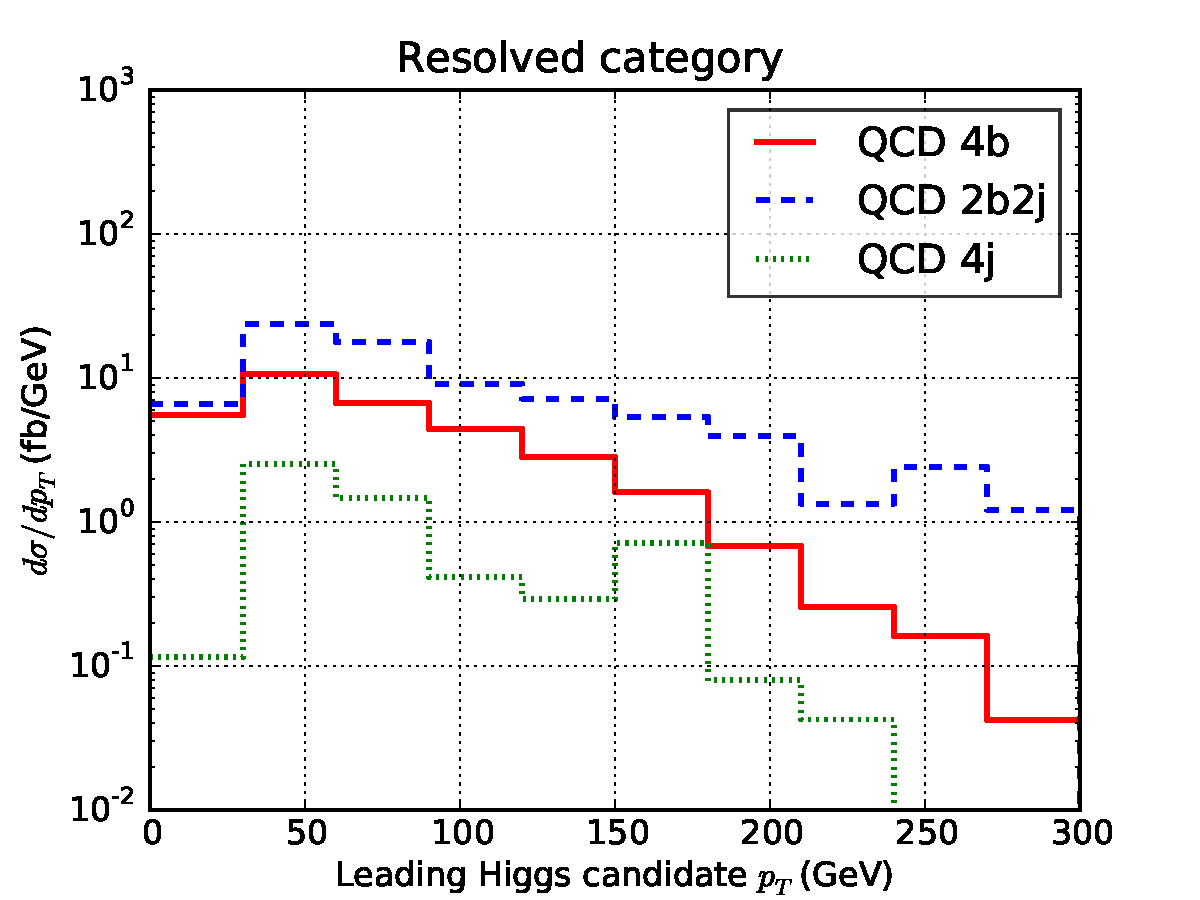
\includegraphics[width=0.49\textwidth]{plots/pt_H0_C2_res_back.pdf}
 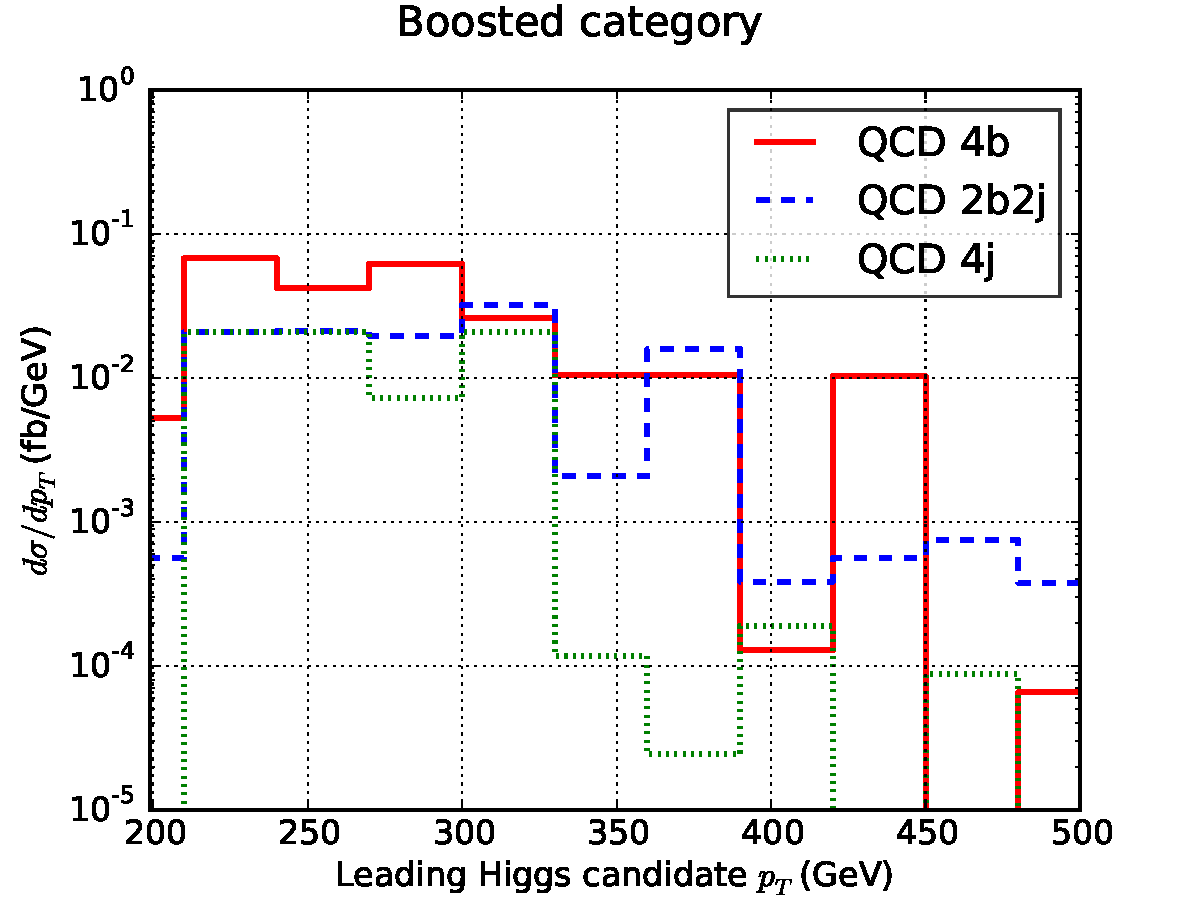
\includegraphics[width=0.49\textwidth]{plots/pt_H0_C2_boost_back.pdf}
   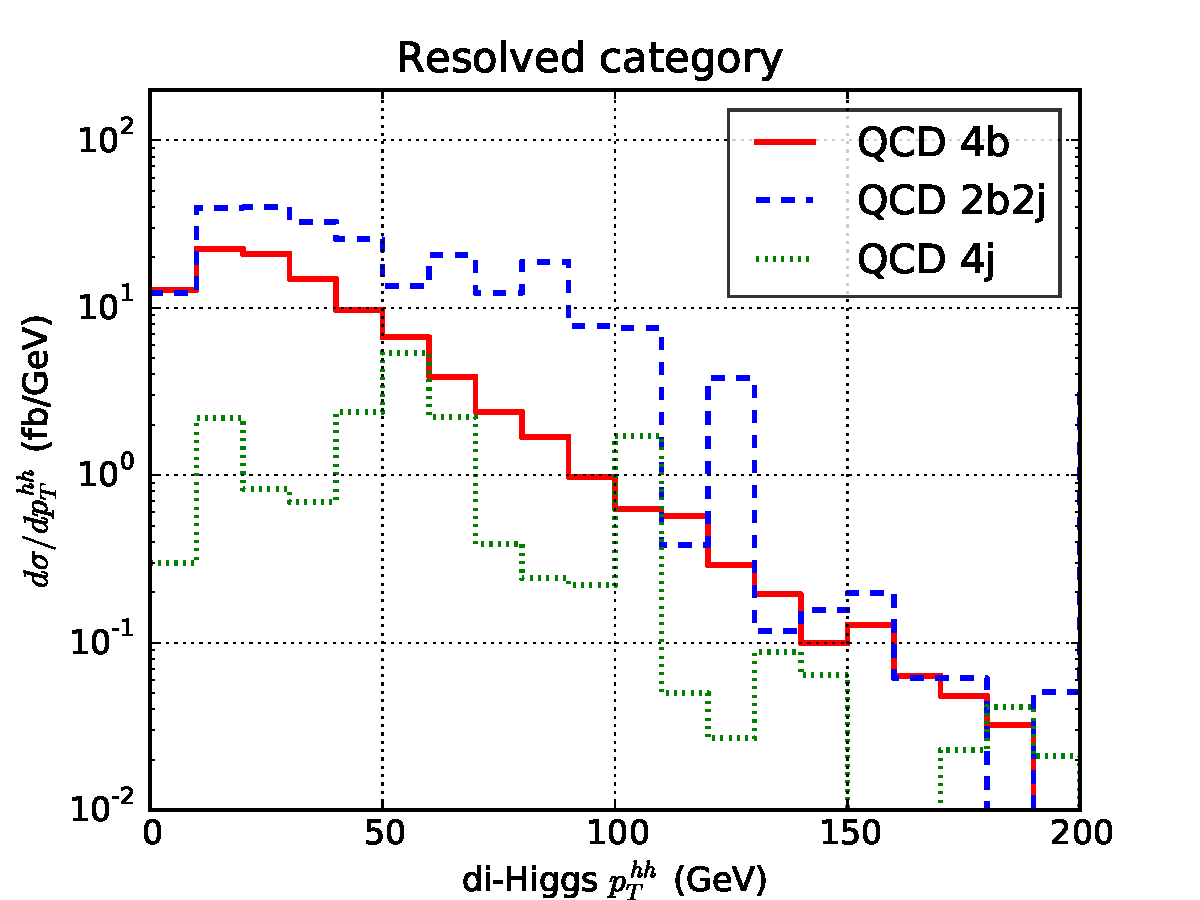
\includegraphics[width=0.49\textwidth]{plots/pt_HH_C2_res_back.pdf}
  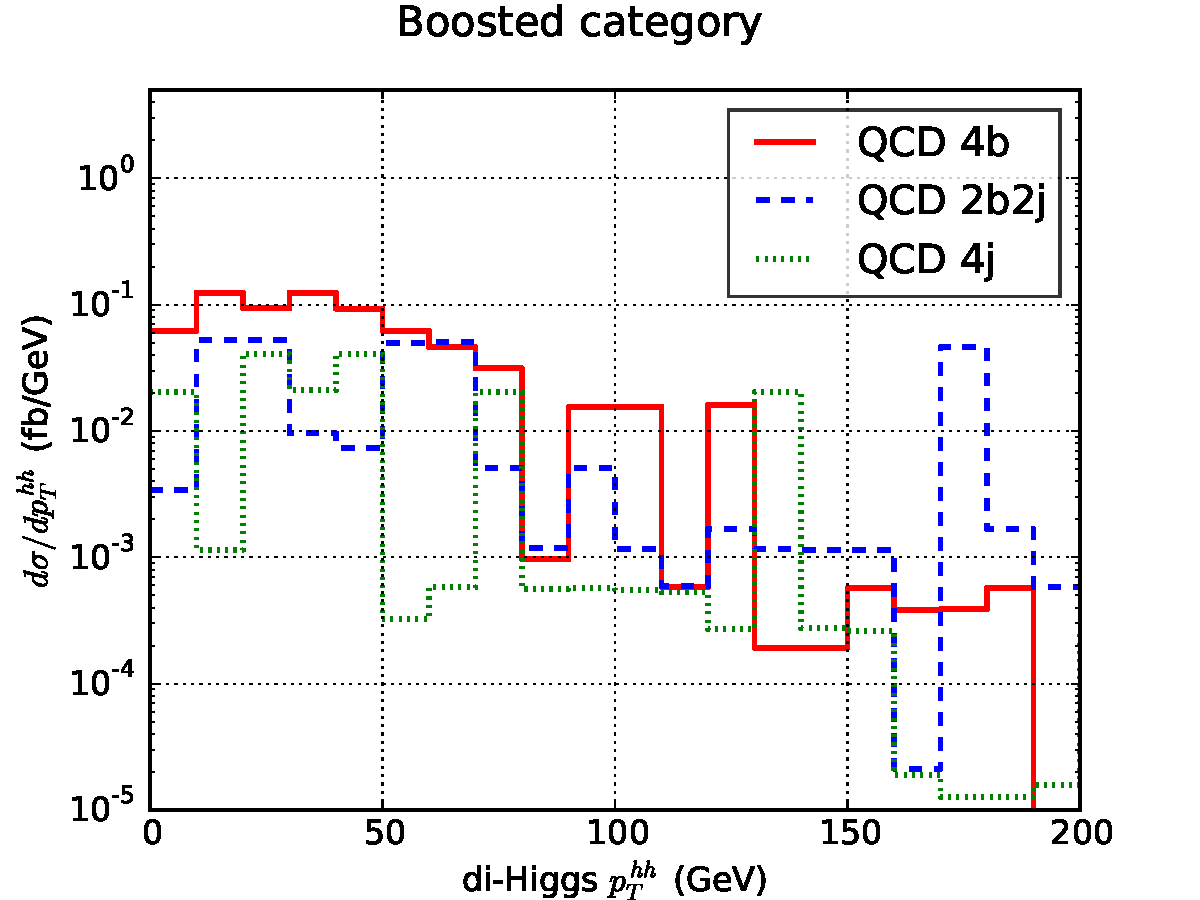
\includegraphics[width=0.49\textwidth]{plots/pt_HH_C2_boost_back.pdf}
  \caption{\small
    Upper plots: the decomposition of the QCD multijet background in its various
    components, $4b$, $2b2j$ and $4j$, for the $p_T$ of the leading
    Higgs candidate in the boosted (left plot) and resolved (right plot) categories.
    %
    Lower plots: the same comparison this time for the $p_T^{hh}$ of the
    reconstructed di-Higgs system.
}
\label{fig:histoBack}
\end{center}
\end{figure}
%%%%%%%%%%%%%%%%%%%%%%%

  One might ask why the $2b2j$ process
  is not subdominant as compared to $4b$: while its generator-level cross-section is
  much larger, $\sigma_{2b2j} \simeq 240\sigma_{4b}$, one expects a suppression
  of the order of $f_l^2 =10^{-4}$ since only with two light jets mistagged as $b$-jets the event
  would be identified as a Higgs candidate.
  %
  We have checked that this expectation is true only at parton level: once parton shower effects
  are accounted for, both the radiation of $b\bar{b}$ pairs from the shower and combinatorics increase
  the number of $b$ quarks in the final state, enhancing substantially the $2b2j$ rates as compared
  to the naive parton level expectation.
  %
  To verify this, we plot the number of $b$-quarks.....

  {\bf compare parton level with hadron level distributions}


